% !TEX encoding = UTF-8 Unicode
%!TEX root = thesis.tex
% !TEX spellcheck = en-US
%%=========================================



\chapter{Results}\label{chap:results}




The results in this research project are mainly gathered from the final test session, which was held after the last development stage, thus the results reflect the state of the application at the end of the research. 

The test sessions had two separate formal data gathering strategies: 

A knowledge test taken by the test participants before and after the session,  this was meant to demonstrate learning value in short term time frame. Such a simple short term test could support the claim that the artifact can be used as an educational tool, 


% though further research is needed.

\section{Learning value}

\section{Usability}


% % The result of this project is the preliminary work for my master thesis next semester, thus 

% \section{Nevrolens}\label{nevrolens}
% Nevrolens is the name I've given the application which is the research product of this project. It's a combination of the Norwegian word Nevroanatomi and HoloLens. It is a AR application running on HoloLens 1, HoloLens 2 and Android. 

% The application is focused on delivering a single user experience, with features as cutting planes, scaling, moving brain parts and transparent brain parts. \autoref{fig:nevrolens_holo} show these features running on HoloLens 2, while \autoref{fig:nevrolens_android} show them on Android.
% It is packages and released on GitLab at \url{https://gitlab.stud.idi.ntnu.no/imtel/nevrolens}. 

% \begin{figure}[h]\label{fig:nevrolens_holo}
%     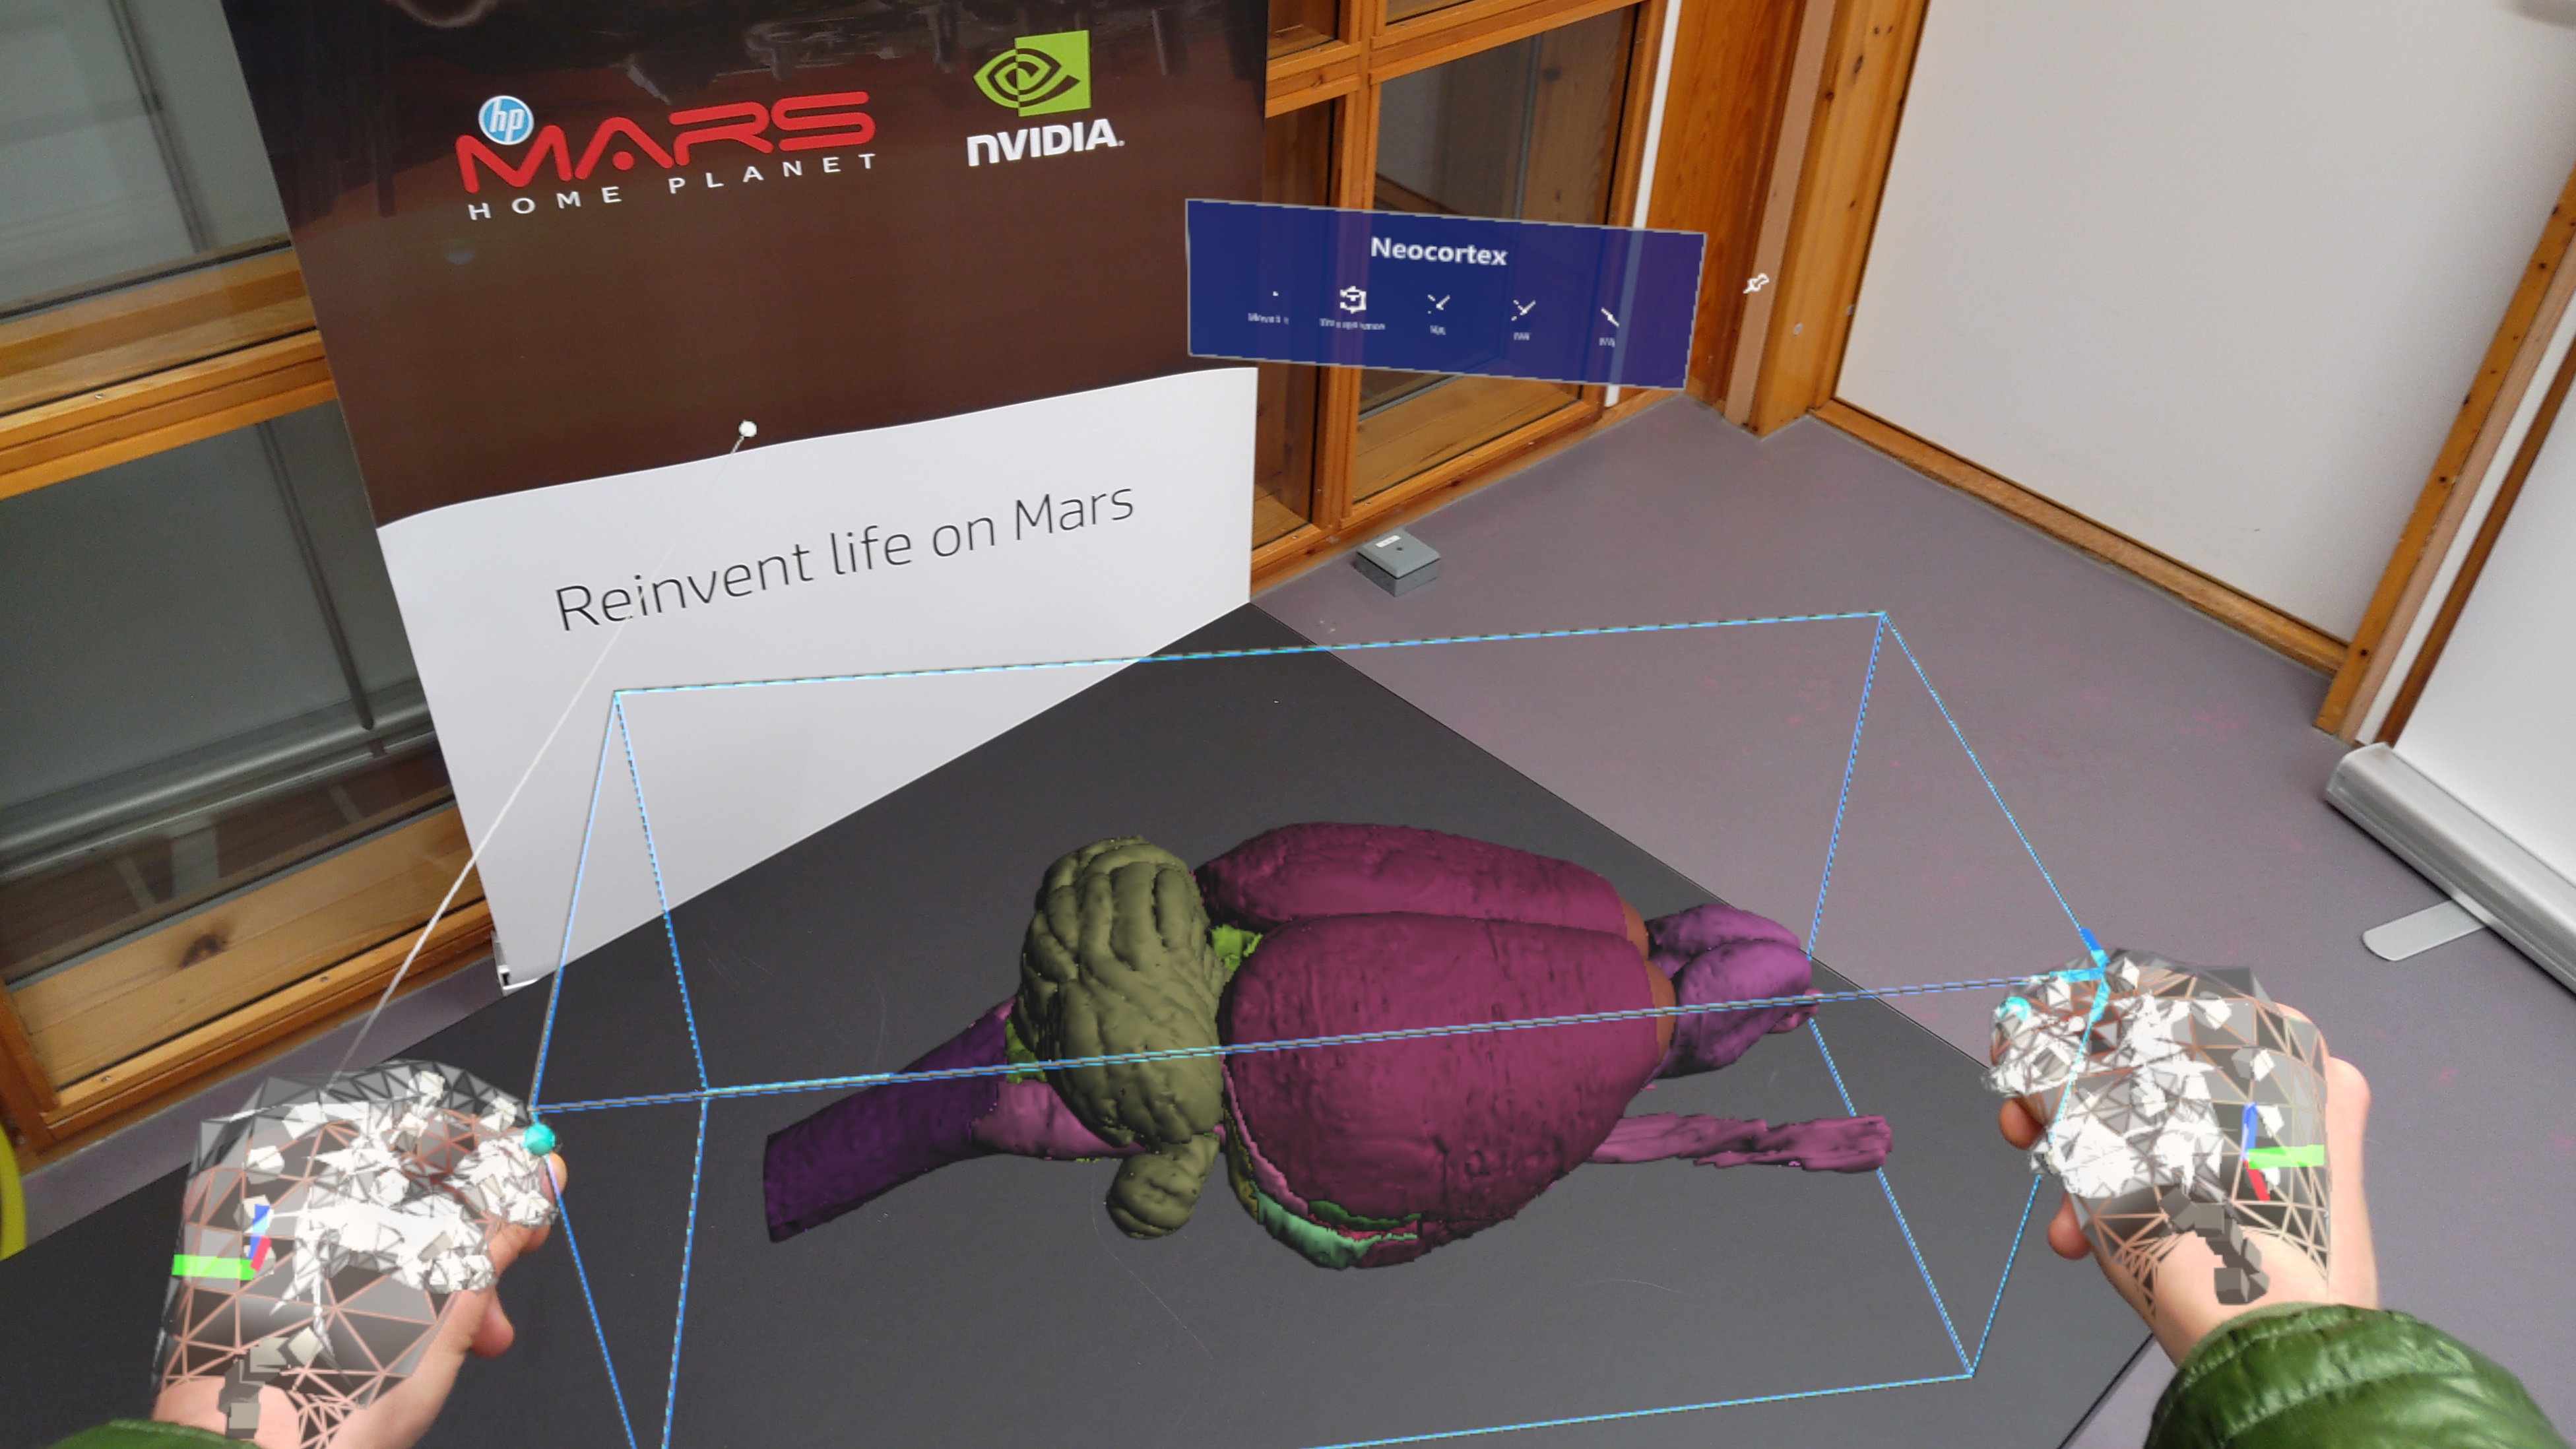
\includegraphics[width=0.5\textwidth]{fig/nevrolens/twohandedzoom.jpg}
%     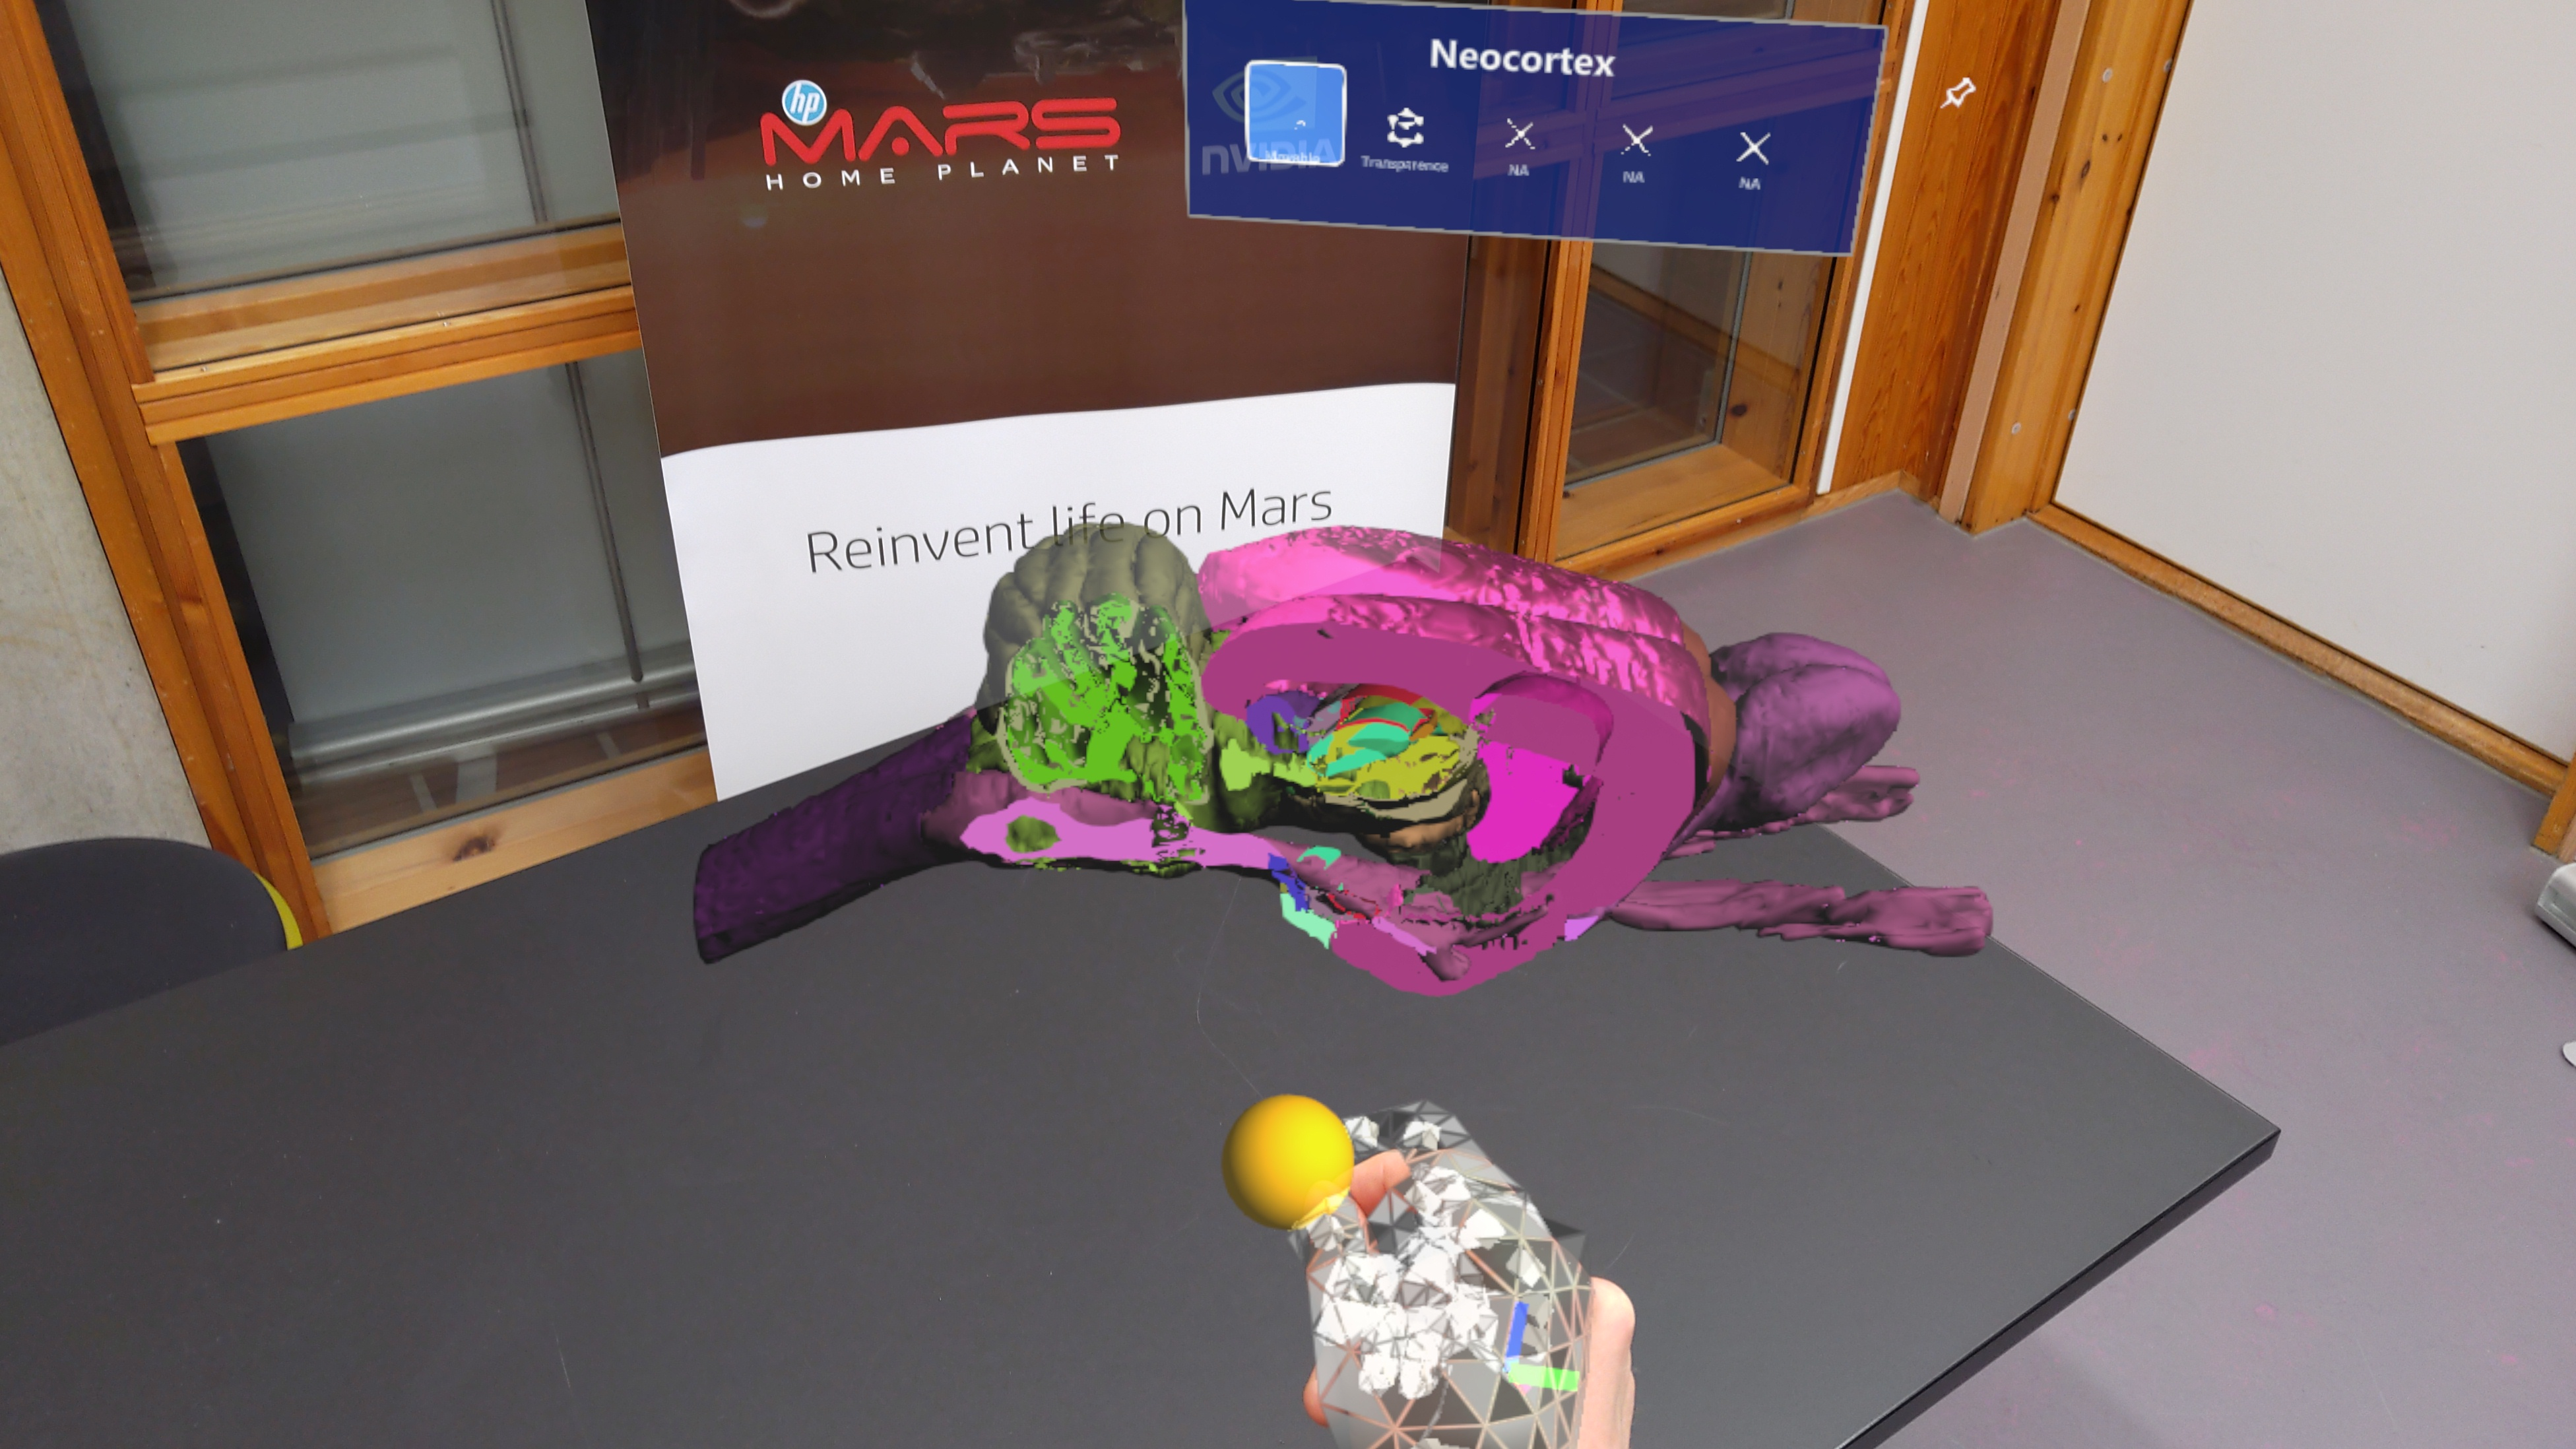
\includegraphics[width=0.5\textwidth]{fig/nevrolens/clipping.jpg}
%     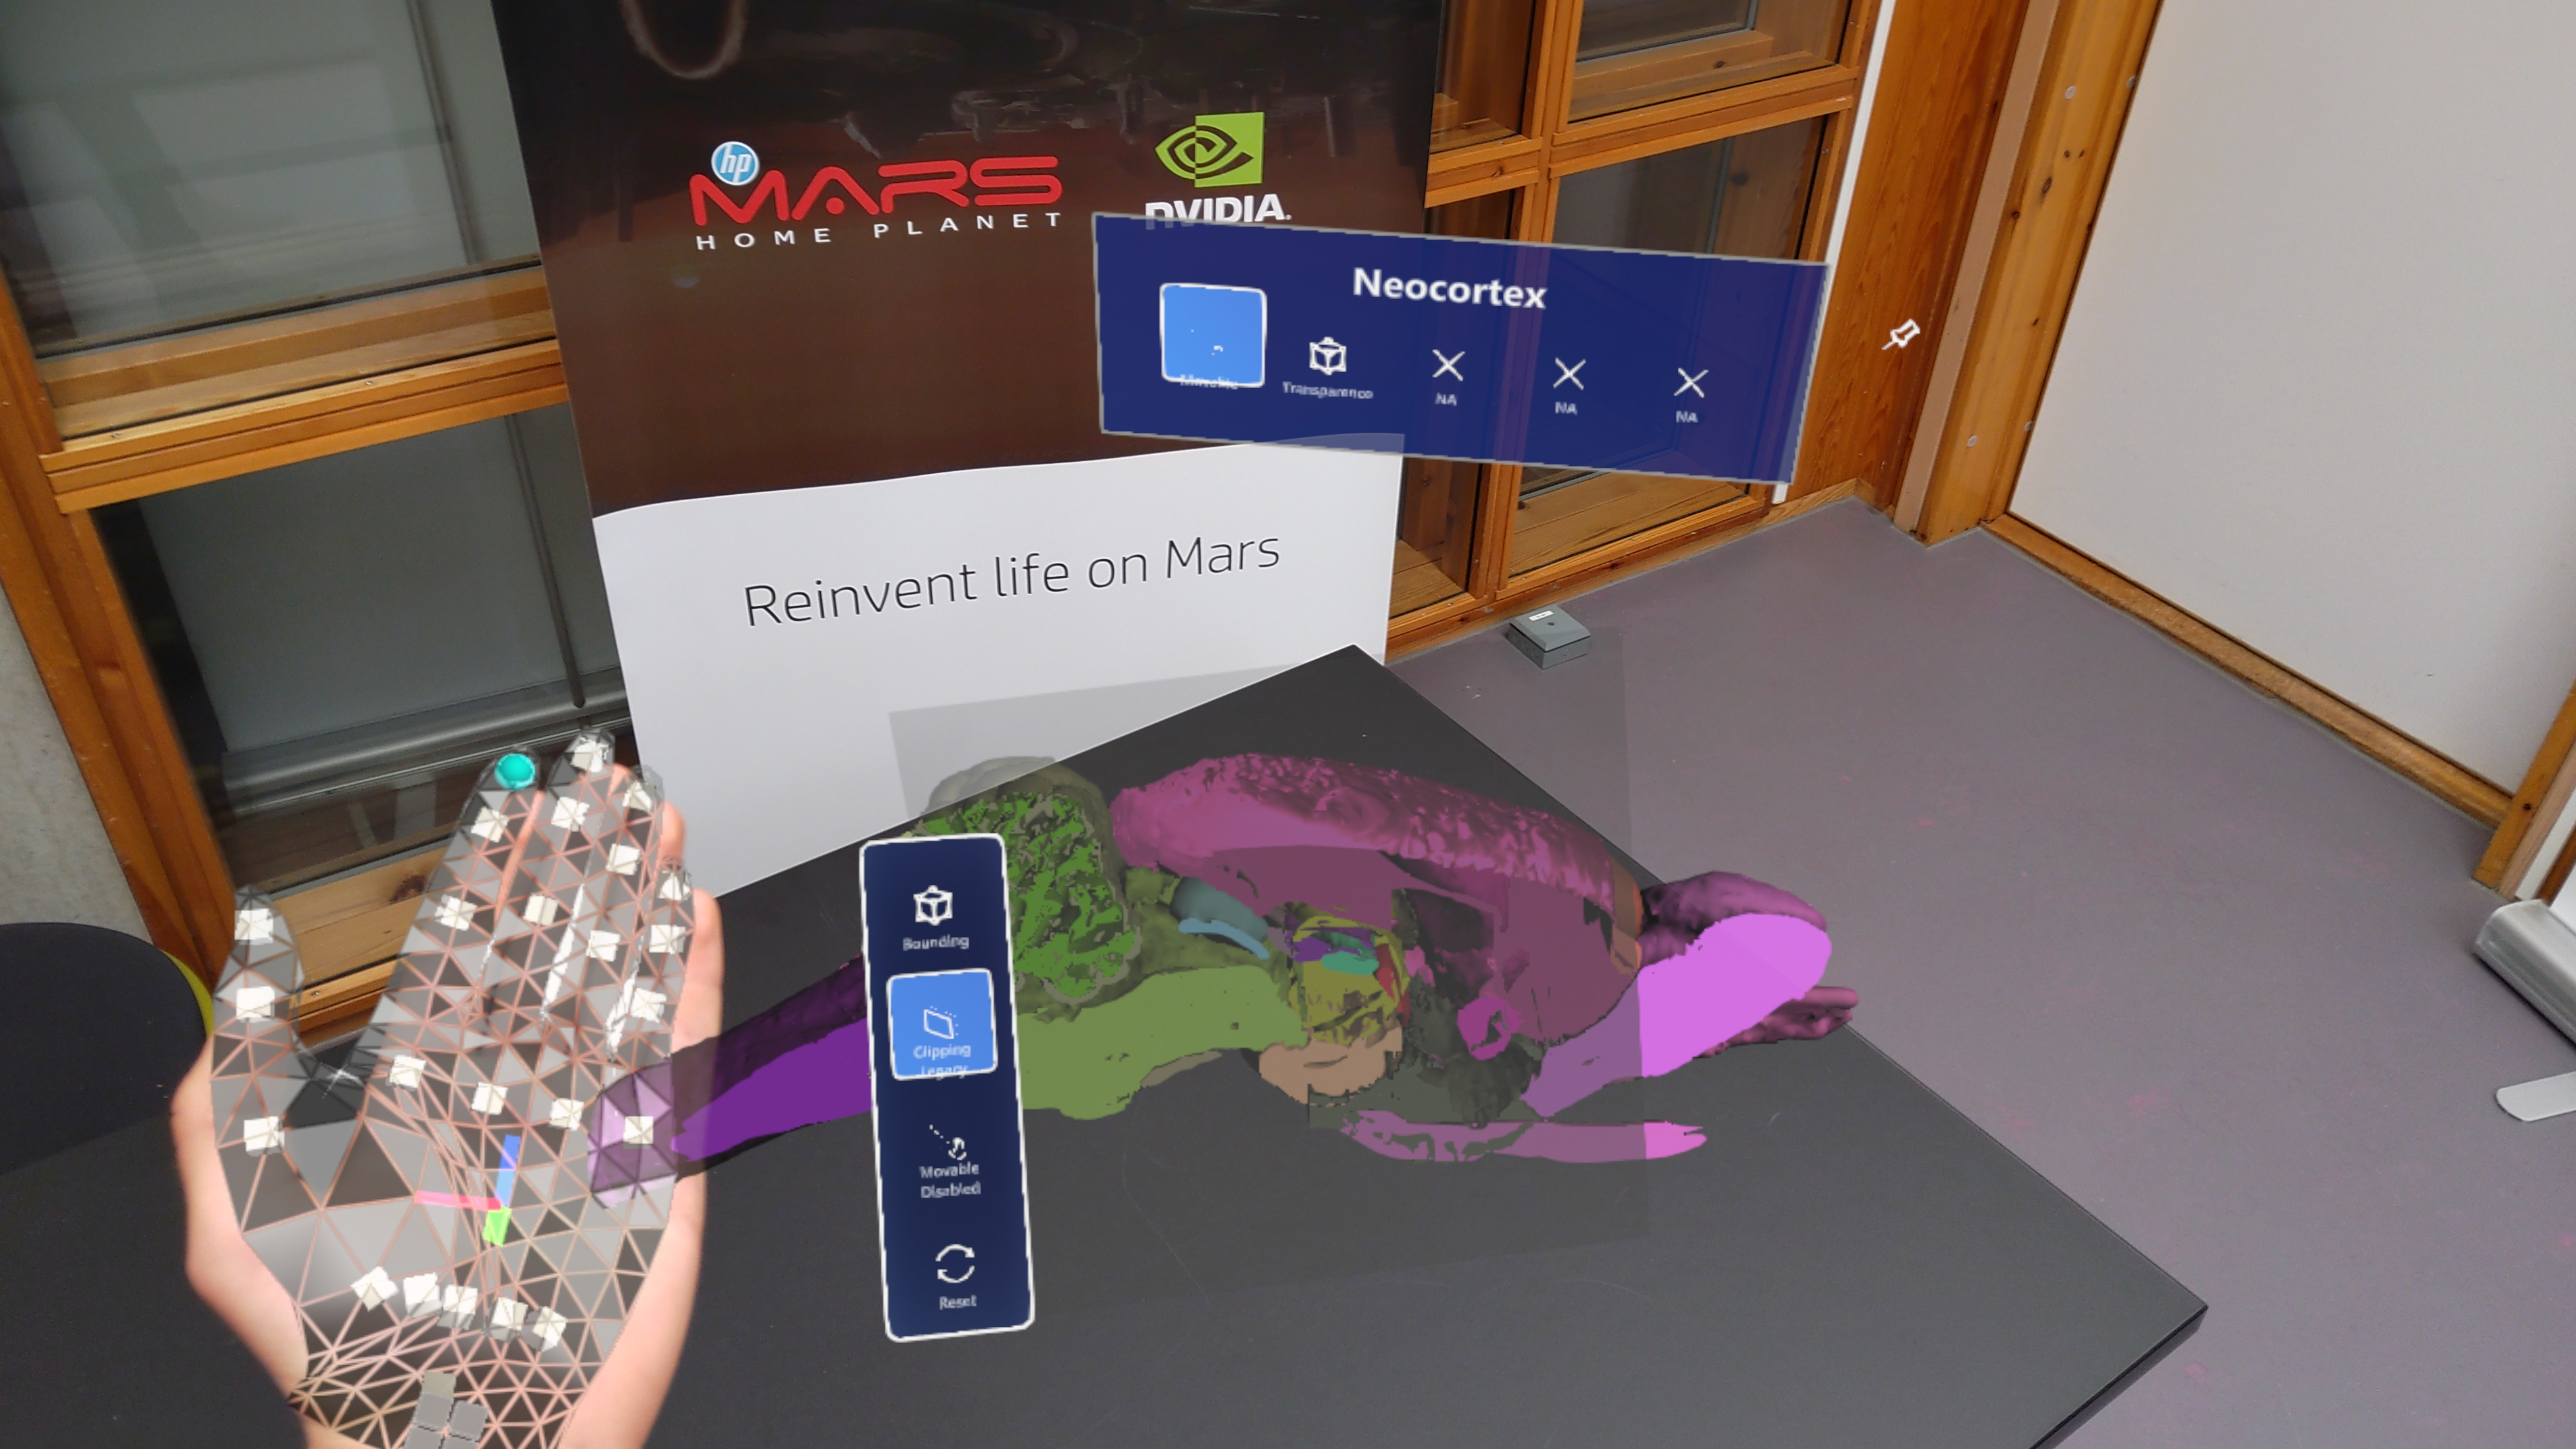
\includegraphics[width=0.5\textwidth]{fig/nevrolens/palmmenu.jpg}
%     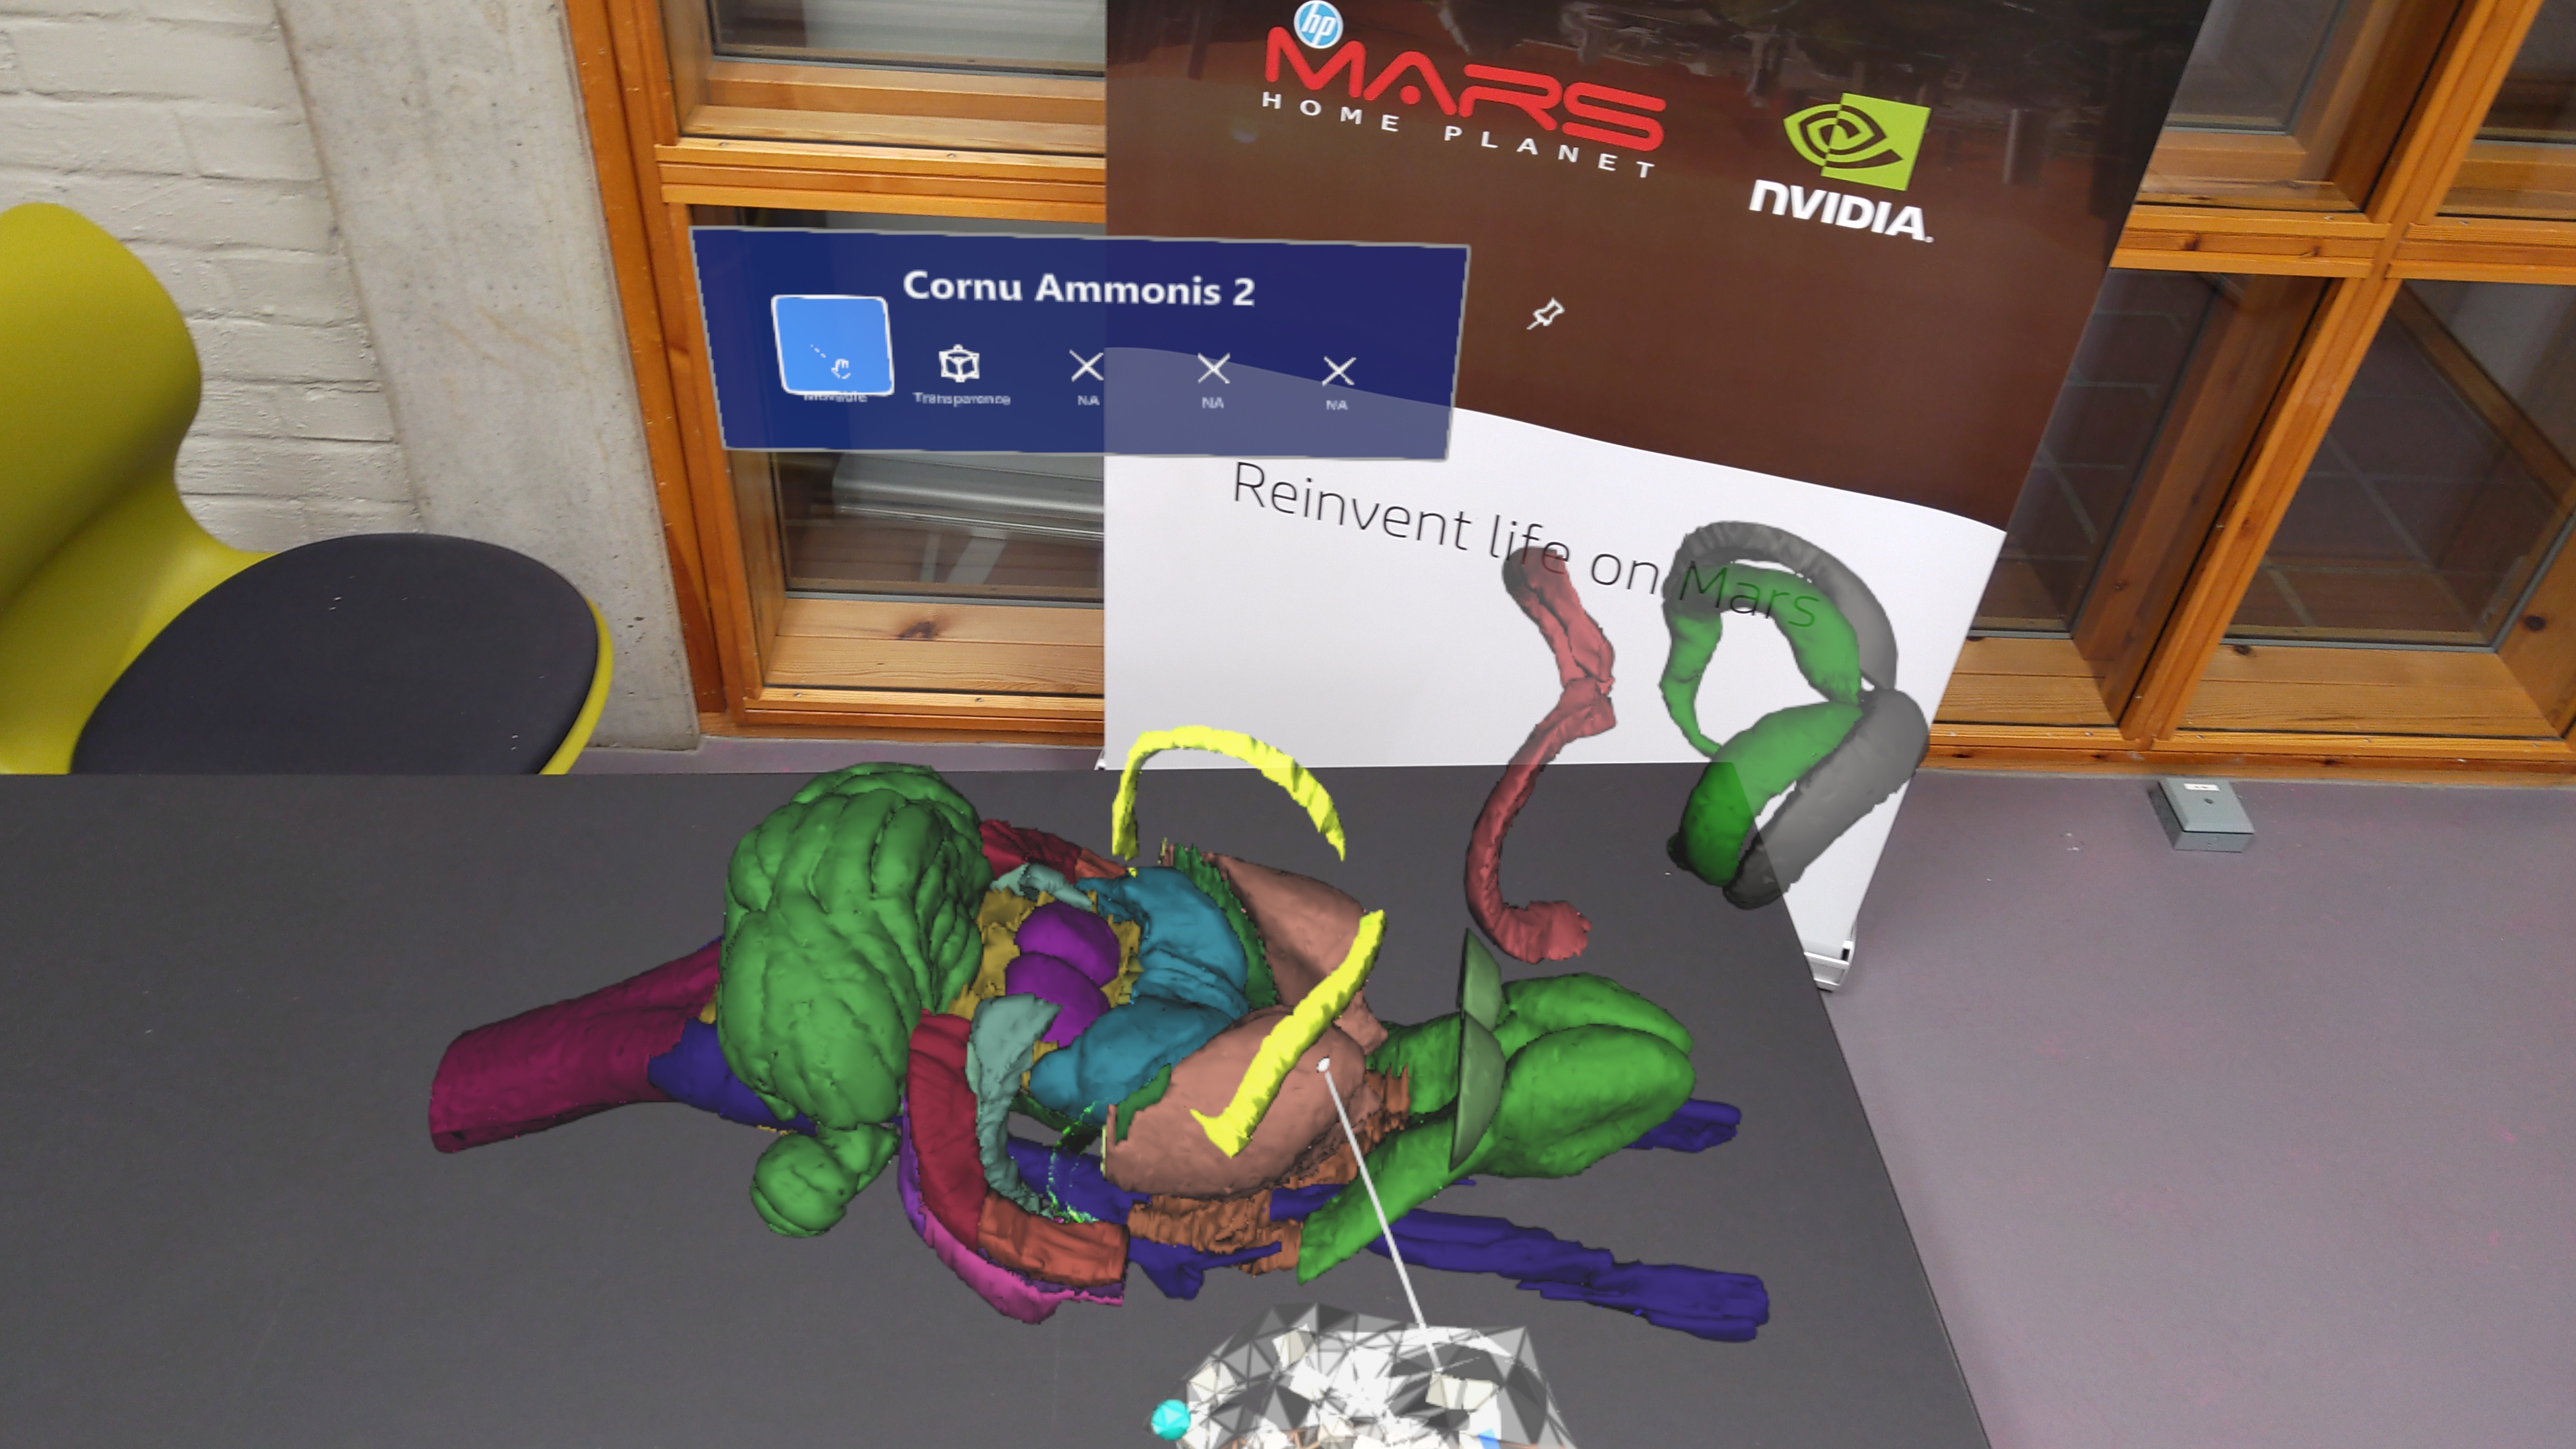
\includegraphics[width=0.5\textwidth]{fig/nevrolens/brainpartsout.jpg}
%     \caption{Nevrolens v0.1.3 on HoloLens 2}
% \end{figure}


% \begin{figure}[h]\label{fig:nevrolens_android}
%     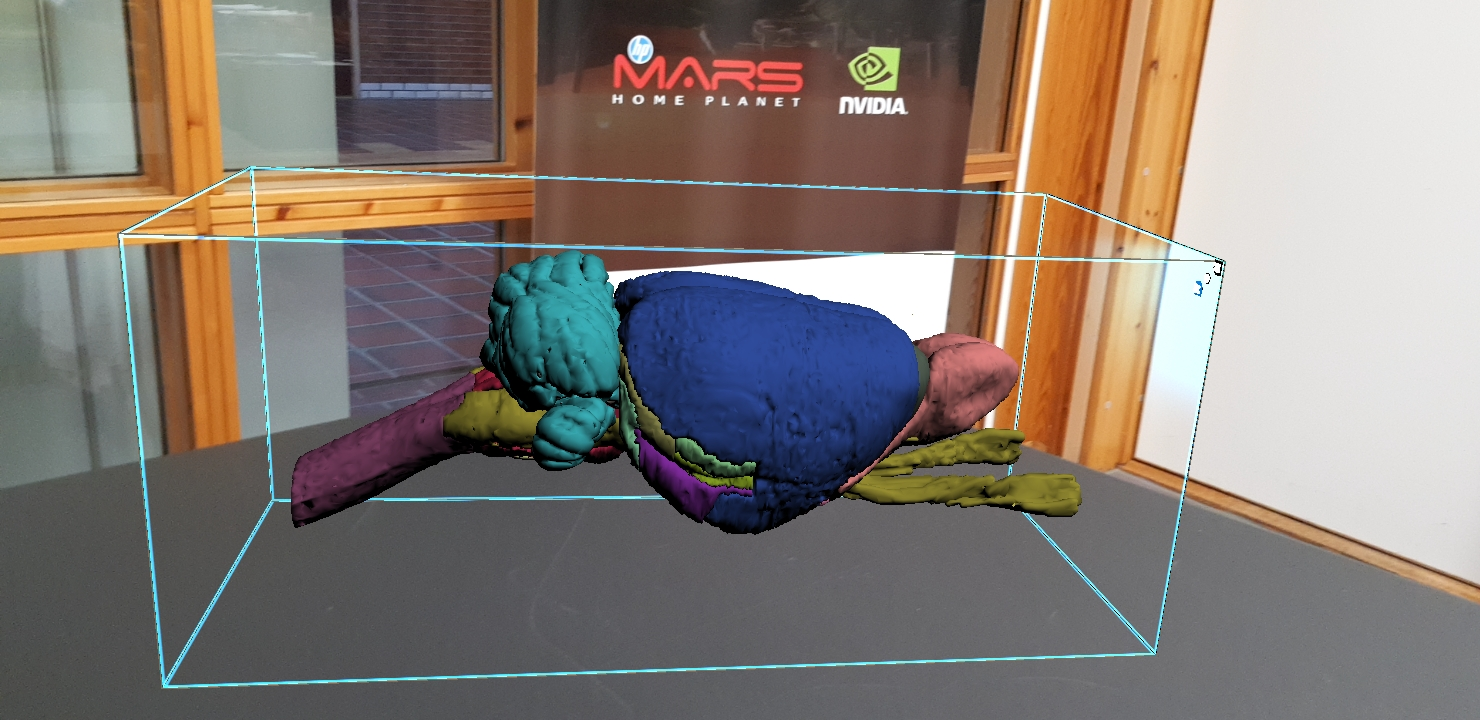
\includegraphics[width=0.5\textwidth]{fig/nevrolens/android_zoom_large.jpg}
%     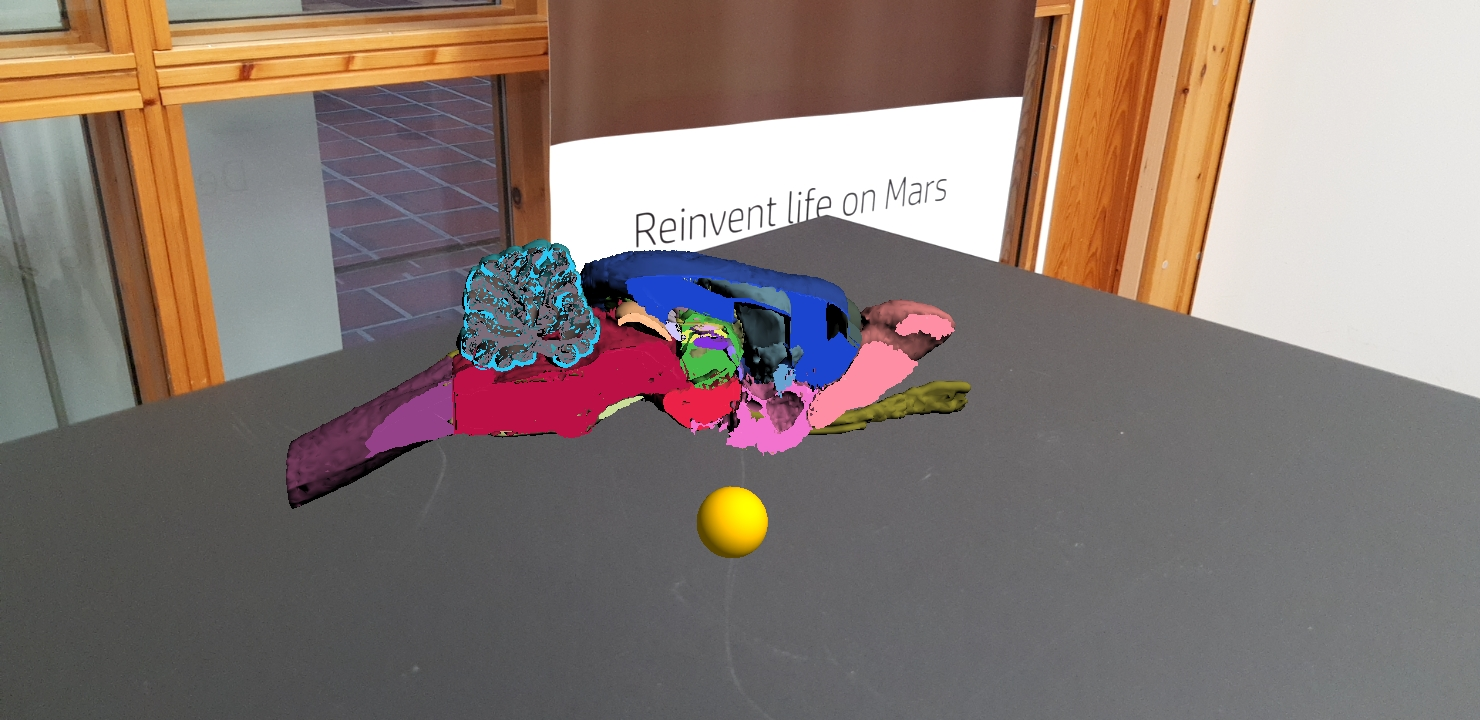
\includegraphics[width=0.5\textwidth]{fig/nevrolens/android_clipping.jpg}
%     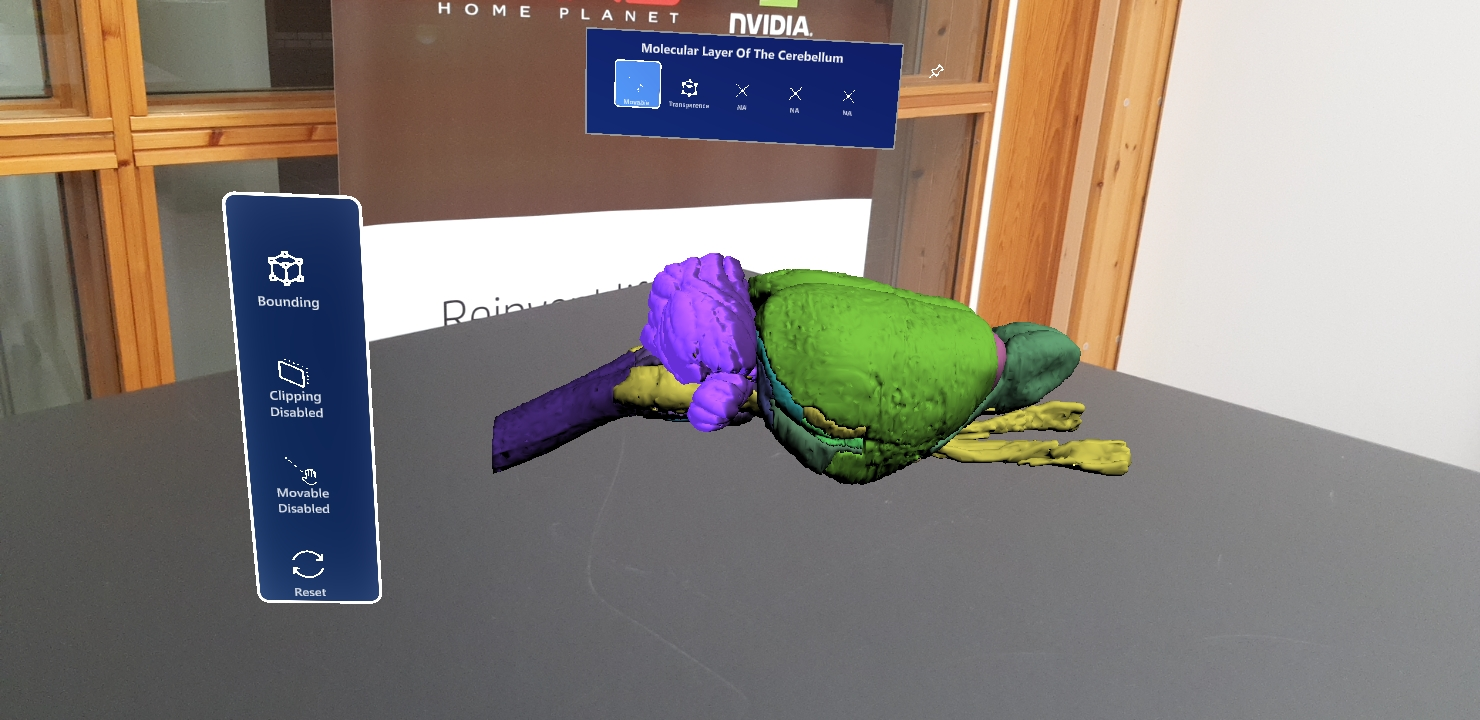
\includegraphics[width=0.5\textwidth]{fig/nevrolens/android_palmmenu.jpg}
%     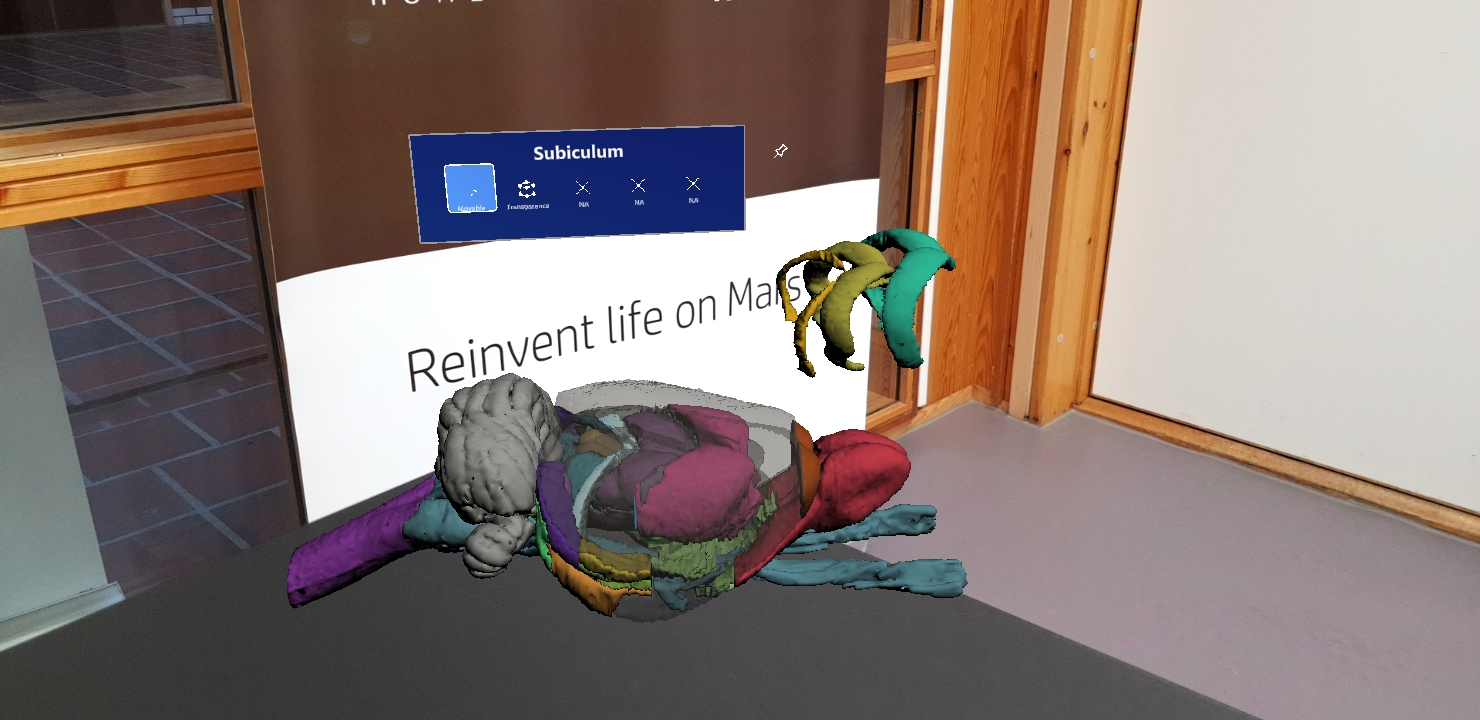
\includegraphics[width=0.5\textwidth]{fig/nevrolens/android_partsout.jpg}
%     \caption{Nevrolens v0.1.3 on Android}
% \end{figure}





% \section{Results}

% Because of the COVID-19 pandemic no user testing has been done this semester, in fact no medical students or professionals have tried the application in-person. Thus, it has been difficult to do formal interviews or gather much feedback, especially regarding interaction. This project is the preliminary work for my master thesis next semester and result gathering will naturally be a much more in focus then. And though no user testing has found place, we have arranged live demoes with \nameref{chap:wdp} over Zoom, which have generated useful feedback. 
% In one such demonstration, I wore a HoloLens 2 and use Nevrolens with guidance from a neuroscientist to extract related regions of the brain and was lectured on their role in behavior. 
% The feedback on its use for a single user, was that there should be a global list menu to toggle different features on each brain part, that there should be ability to increase resolution of a single brain part and some way to visualize microscopical data. 

% % Mostly, the feedback has been positive

% % Success in picking out brain parts, and explaining different structures in the brain. 



% % results from this project are limited.